\chapter{Étude de l’existant}

    E-Yaka est un \emph{serious game} destiné à former les étudiants à la gestion d'une entreprise. À destination des écoles, ce simulateur de gestion permettra à plusieurs équipes d'entrer en concurrence sur un même marché.

    \section{Serious game}

        Un \emph{serious game} est une application informatique dont l'objectif est de combiner des aspects sérieux comme l'enseignement, la communication, ou encore l'information, avec des ressorts ludiques issus du jeu vidéo. Une telle association a donc pour but de s'écarter du simple divertissement.

        Plus particulièrement, un \emph{serious game} est un outil d’apprentissage utilisant les nouvelles technologies afin de faire passer un message de manière attractive. L’intention de ce message peut être pédagogique, informative, publicitaire, communicative. Le \emph{serious game} conserve par conséquent l’aspect ludique des jeux vidéos classiques.

        Un \emph{serious game} a pour principal objectif de sensibiliser, de faire apprendre, de communiquer, d’informer, de faire passer un message publicitaire ou encore d’entraîner physiquement ou mentalement l’apprenant. Ces logiciels sont présents dans pratiquement tous les domaines professionnels : gouvernement, armée, santé, entreprise, politique, médias...

        Le nombre d’entreprises utilisant les \emph{serious games} ne cesse de croître car ces entreprises veulent pouvoir simuler l’activité sans prise de risques. La plupart d'entre elles n’ont pas à leur disposition des simulateurs sur mesure avec des données de marché réelles, dont les actions n'ont pas d'impact direct sur les activités de l’entreprise. Les \emph{serious games} peuvent servir de simulateur pour ces entreprises. Ils permettent donc aux utilisateurs de mettre en pratique leurs compétences sans risque quelconque.

        Les \emph{serious games} à but pédagogique, tels que E-Yaka, mettent en avant l’aspect pédagogique ou éducatif au sein du jeu : \enquote{apprendre en s’amusant}. Un des principaux avantages du \emph{serious game} est évidemment l’impact positif sur la motivation des apprenants. Il est légitime de penser que l’introduction du jeu dans le milieu éducatif produit un effet de nouveauté qui ne sera que temporaire, cependant plusieurs études montrent bien que l’utilisation de \emph{serious games} impacte positivement la motivation des apprenants sur le long terme (Malone, 1981; Wix, 2012).

        Un jeu adapté donne des retours réguliers à l’apprenant sur ses actions, entretenant ainsi sa motivation. Les \emph{serious games} sont basés sur un mode d’apprentissage par essais et erreurs car l’apprenant est amené à construire mentalement une hypothèse qu’il pourra ensuite tester directement dans le jeu. L’apprenant affinera ses hypothèses afin de trouver une stratégie qui lui permette de gagner.

        Enfin, les \emph{serious games} permettent de prendre en compte les différences de rythme d’apprentissage entre apprenants. Un apprenant qui a besoin de répéter une séquence plusieurs fois dans le but de mieux comprendre a tout à fait la possibilité de le faire. Et à l’inverse, un apprenant qui aurait assimilé les concepts du premier coup ne serait pas dans l’obligation d’attendre les autres.

    \section{Business game}

        Les \emph{business games} ou jeux de simulation d’entreprise sont des \emph{serious games} à but pédagogique construits sous la forme d’un jeu de rôle. Ces jeux s’appuient sur un logiciel modélisant un environnement concurrentiel et sur les actions des entreprises dans cet environnement. Les entreprises en question sont gérées par les joueurs, qui sont généralement regroupés au sein d’équipes concurrentes.

        L’apprenant devient alors acteur de sa formation, il est au centre du cycle de décisions et est libre de choisir sa propre stratégie afin de mener son entreprise à la réussite. Le fait de pouvoir recommencer un nouveau cycle à chaque fois permet d’apprendre en manipulant. Le jeu de simulation d’entreprise est utilisé sur des sujets tels que l’économie, le marketing, l’innovation, la gestion de projet...

        E-Yaka, le jeu auquel nous nous intéressons pour l’analyse de traces, est l'un de ces jeux de simulation d’entreprise.


    \section{Principe et fonctionnalités de l'application E-Yaka}

        E-Yaka est un simulateur d'entreprise programmé en \emph{PHP} avec le framework \emph{Symfony2}. Ce simulateur se présente sous la forme d'une compétition entre différentes entreprises naissantes. Chaque entreprise est gérée par un groupe d'étudiants qui cherche à avoir de meilleurs résultats que les autres groupes participant à la même partie. Le jeu se divise en plusieurs tours représentant chacun une année de l'entreprise. Ces années sont découpées en plusieurs cycles de prospection, dont le nombre peut être choisi par l'animateur au lancement de la partie. Entre chaque tour, les équipes prennent des décisions de gestion favorisant la compétitivité de leur entreprise.
    
        Avant la partie, l'animateur renseigne un certain nombre de paramètres tels que la durée des cycles et des tours, les taux (de TVA par exemple), les amortissements, les pourcentages de répartition du résultat, etc.

        De plus, l'animateur donne des précisions sur le produit qui sera proposé à la vente par toutes les entreprises en jeu (différentes formules, prix, frais d'installation, de déplacement...) ainsi que sur les prospects (leurs noms, leurs secteurs respectifs...). Puis l'animateur peut paramétrer le prix à l'achat d'information sur les prospects à destination des apprenants.

        Durant la partie, l'animateur décide quand changer de cycle ou quand passer au tour suivant. Il peut aussi se connecter à la partie comme s'il était membre d'une entreprise, et prendre des décisions comme un joueur pourrait le faire.
        L'animateur peut envoyer des messages aux joueurs sous forme de notifications et peut aussi préparer des questionnaires qui seront envoyés aux joueurs au début d'un tour donné, comme présenté sur l'image \ref{questionnaire}.

        \begin{figure}
        	\centering
            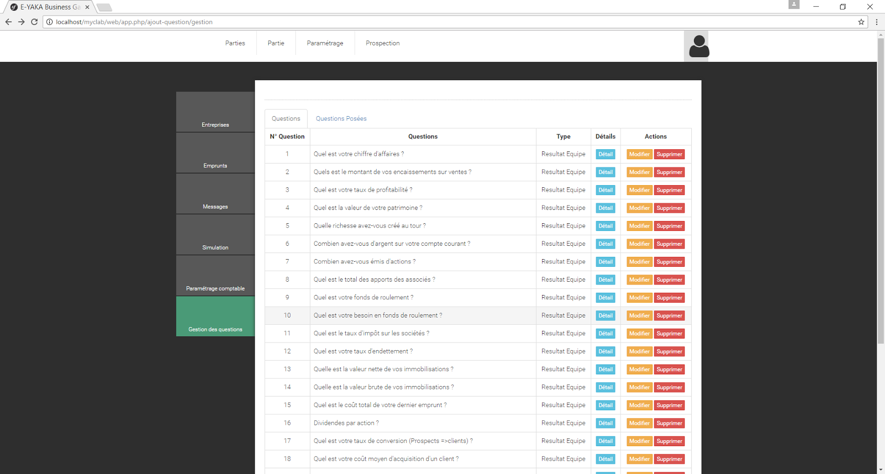
\includegraphics[scale=0.88]{images/questionnaire.png}
            \caption{Gestion des questions}
            \label{questionnaire}
        \end{figure}


        Enfin, l'animateur a accès à tout moment à un bilan détaillé de chacune des entreprises, et c'est notamment lui qui paramètre le premier bilan en début de partie.

        De leur côté, les joueurs doivent gérer au mieux le temps qui leur est imparti à chaque tour de jeu pour faire croître leur entreprise et démarcher un maximum de clients. Ils peuvent notamment acquérir des informations sur les prospects (en les achetant ou en les recherchant directement auprès des entreprises concernées), pour ensuite leur proposer des devis et gagner de nouveaux clients. Ces informations peuvent être qualitatives ou quantitatives, et permettront au joueur d'estimer au mieux le meilleur devis satisfaisant le prospect en fonction du degré d'adoption d'innovation du prospect (\emph{innovator}, \emph{early adopter}...), du prix du produit, du lot vendu, etc.

        Plusieurs options permettent au joueur de gérer sa comptabilité, de visualiser ses parts de marché, son chiffre d'affaires, sa notoriété ou son bilan financier global (voir figure \ref{bilan_financier}). Cela lui permettra de prendre les meilleures décisions pour son entreprise en se basant sur des données économiques tangibles. Il peut par ailleurs obtenir quelques informations sur les entreprises concurrentes.

        \begin{figure}\centering
            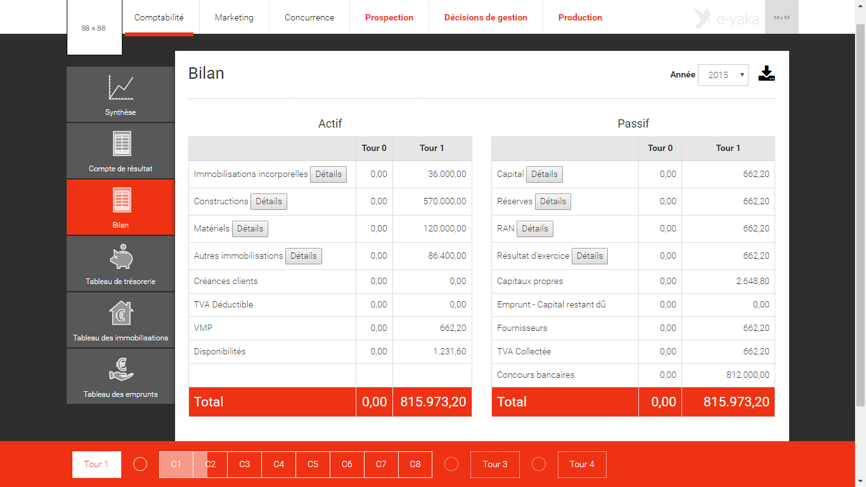
\includegraphics[scale=0.88]{images/bilan.png}
            \caption{Bilan financier}
            \label{bilan_financier}
        \end{figure}

        Il existe également une gestion de base des ressources humaines (personnel polyvalent, à la fois commercial, technicien, ingénieur) notamment sous la forme de recrutement de nouveaux commerciaux. Il est aussi possible pour le joueur de faire des emprunts auprès des banques définies par l'animateur.

        Pour résumer, les tableaux \ref{menus_animateur} et \ref{menus_joueur} ci-après présentent les différents onglets qui sont présents dans les menus de l'interface de l'animateur et du joueur.

        \begin{figure}\centering
            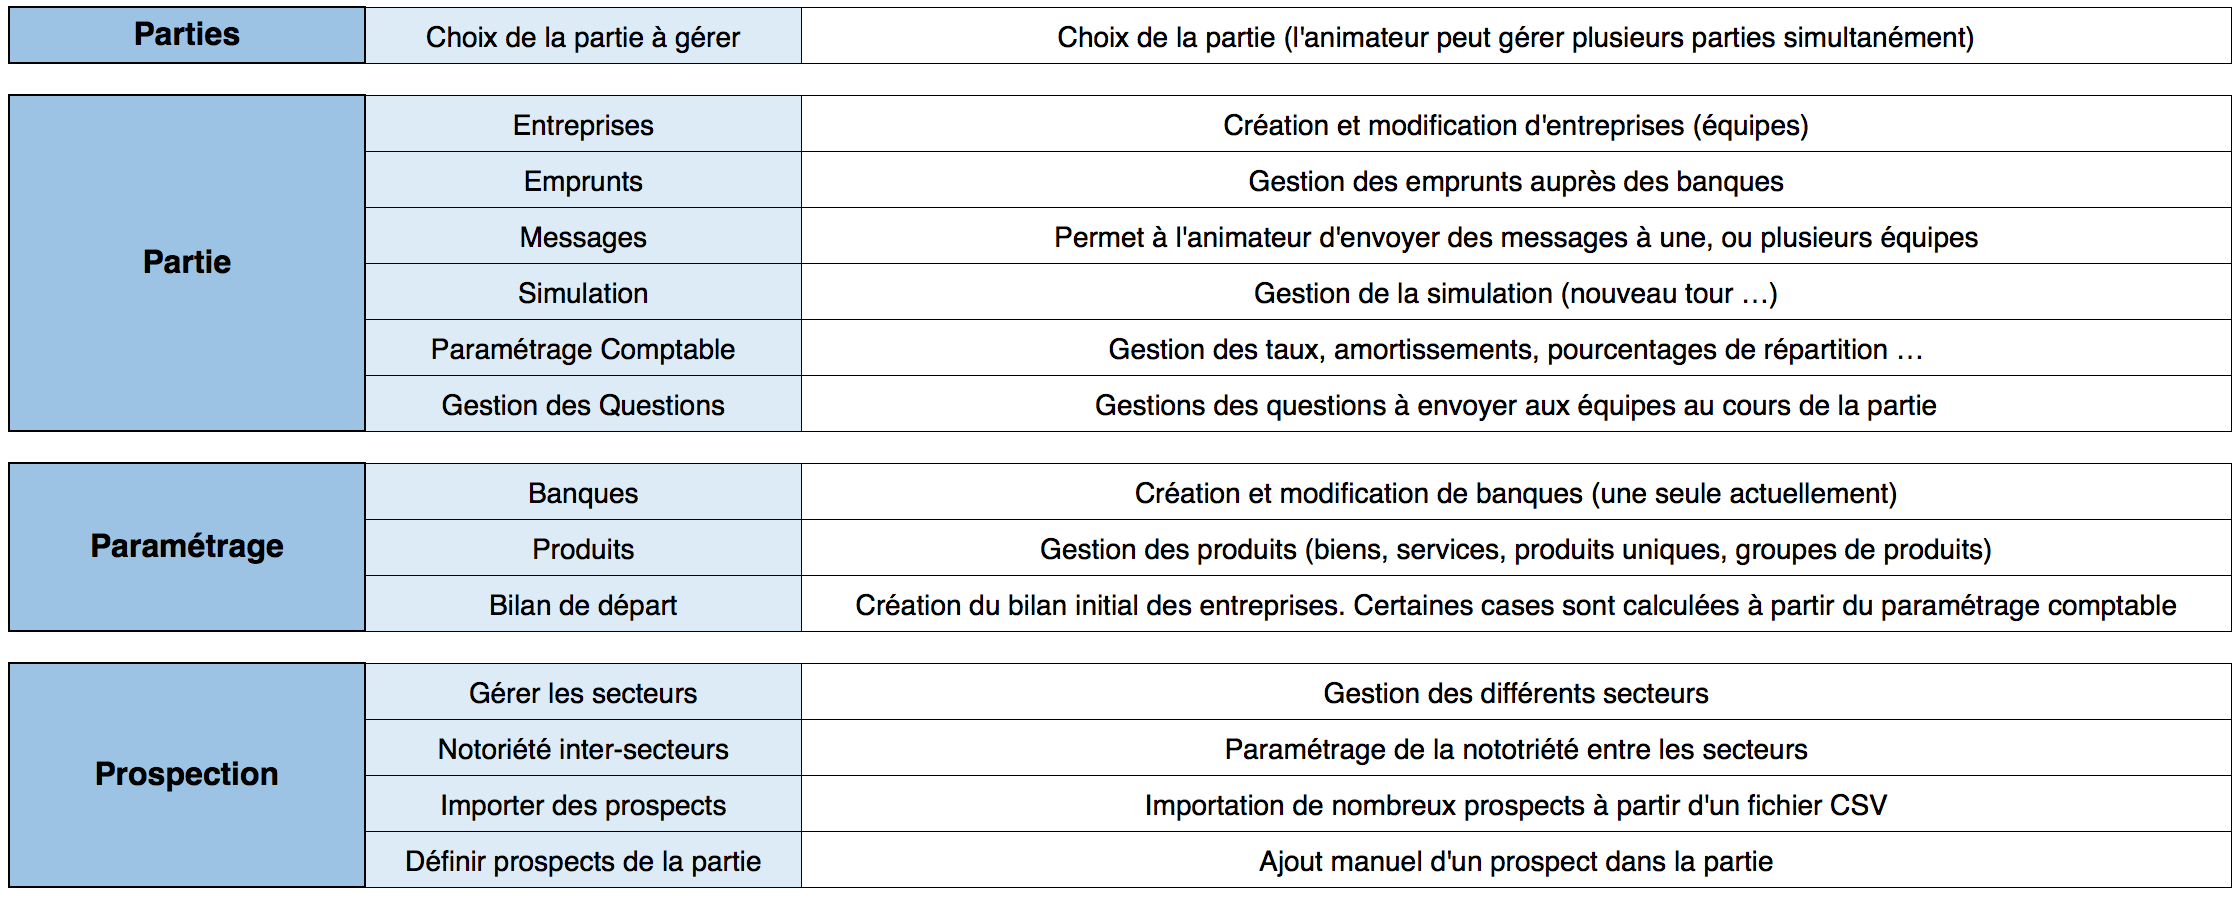
\includegraphics[width=0.9\textwidth]{images/menus_animateur_2.png}
            \caption{Menus de l'animateur}
            \label{menus_animateur}
        \end{figure}

        \begin{figure}\centering
            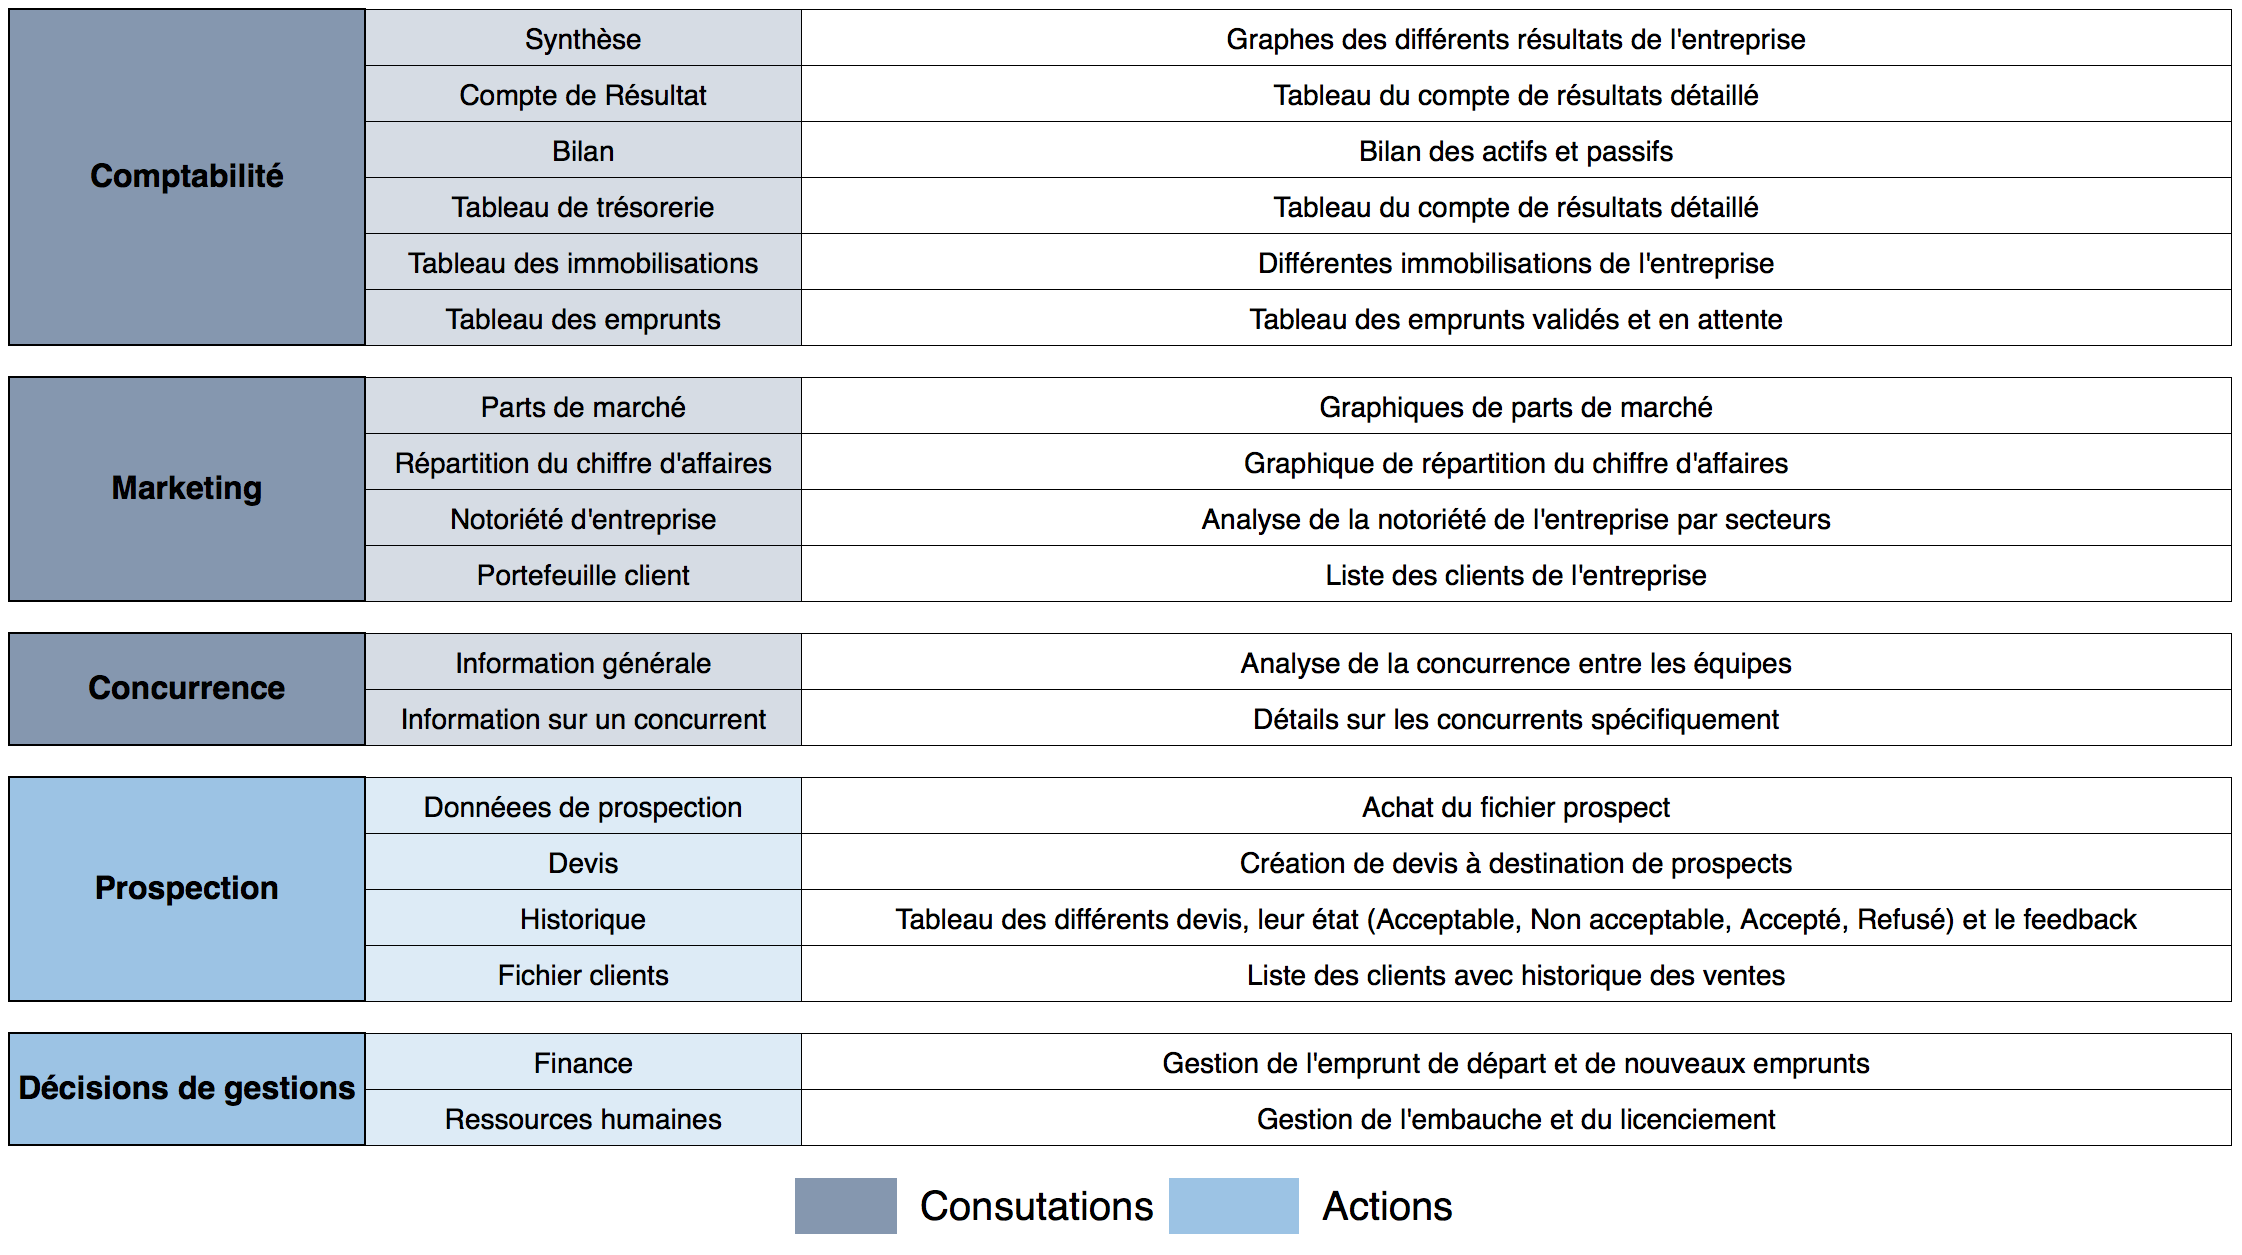
\includegraphics[width=0.9\textwidth]{images/menus_joueur.png}
            \caption{Menus du joueur}
            \label{menus_joueur}
        \end{figure}